\chapter{Results}


Additionally, some other properties and effects that arose during the analysis are also investigated.
\section{Main Results}

\begin{itemize}
    \item Collected change: (Langau fit and most probable value)
    \item Efficiency: (threshold value for the electronics)
    \item Time resolution: (gaussian fit)
\end{itemize}

\subsection{Normal temperature}

\begin{figure}[!ht]
    \centering
    \includegraphics[width=.9\linewidth]{Images/Results/IME_plots_together_voltage_charge_normal_temp.png}
    \caption{}
    \label{fig:normal_temp_IME}
\end{figure}


\subsection{Irradiated}

\begin{figure}[!ht]
    \centering
    \includegraphics[width=.9\linewidth]{Images/Results/IME_plots_together_voltage_charge_irradiated.png}
    \caption{}
    \label{fig:irradiated_IME}
\end{figure}


\subsection{Angled}

\begin{figure}[!hb]
    \centering
    \includegraphics[width=.9\linewidth]{Images/Results/IME_plots_together_angle_charge_normal_temp_voltage:-100.png}
    \caption{}
    \label{fig:angled_IME}
\end{figure}



\section{Detailed analysis}\label{sec:detailed_analysis}

Some other interesting effects that were investigated further.
%%% the titles should be the conclusion, not what I saw:
%%% multiple peaks -> signal from neighbouring pads
%%% - signal from neighbouring pads
%%% - signl from the edges
%%% - effect of the angle of the tracks
%%% - charge sharing (collecting charge collected by the neighbouring pads)
%%% - interpad study?

\subsection{Signal from neighbouring pads}\label{sec:multiple_peaks}

As it was very obvious from Figure \ref{fig:time_cut_gauss+bg_fit}, a second peak appeared in the time distribution.

By picking all the events in a certain time interval and plotting their corresponding reconstructed tracks, we were able to verify that: the main peak simply coincides with the DUT, the second peak arises from events picked up by its neighbouring pad. Figure \ref{fig:time_difference_multiple_peaks_highlight} is evidence of this.
Furthermore, this effect was only observed in DUTs which were part of 2x2 LGAD arrays.

\begin{figure}[!ht]
    \centering
    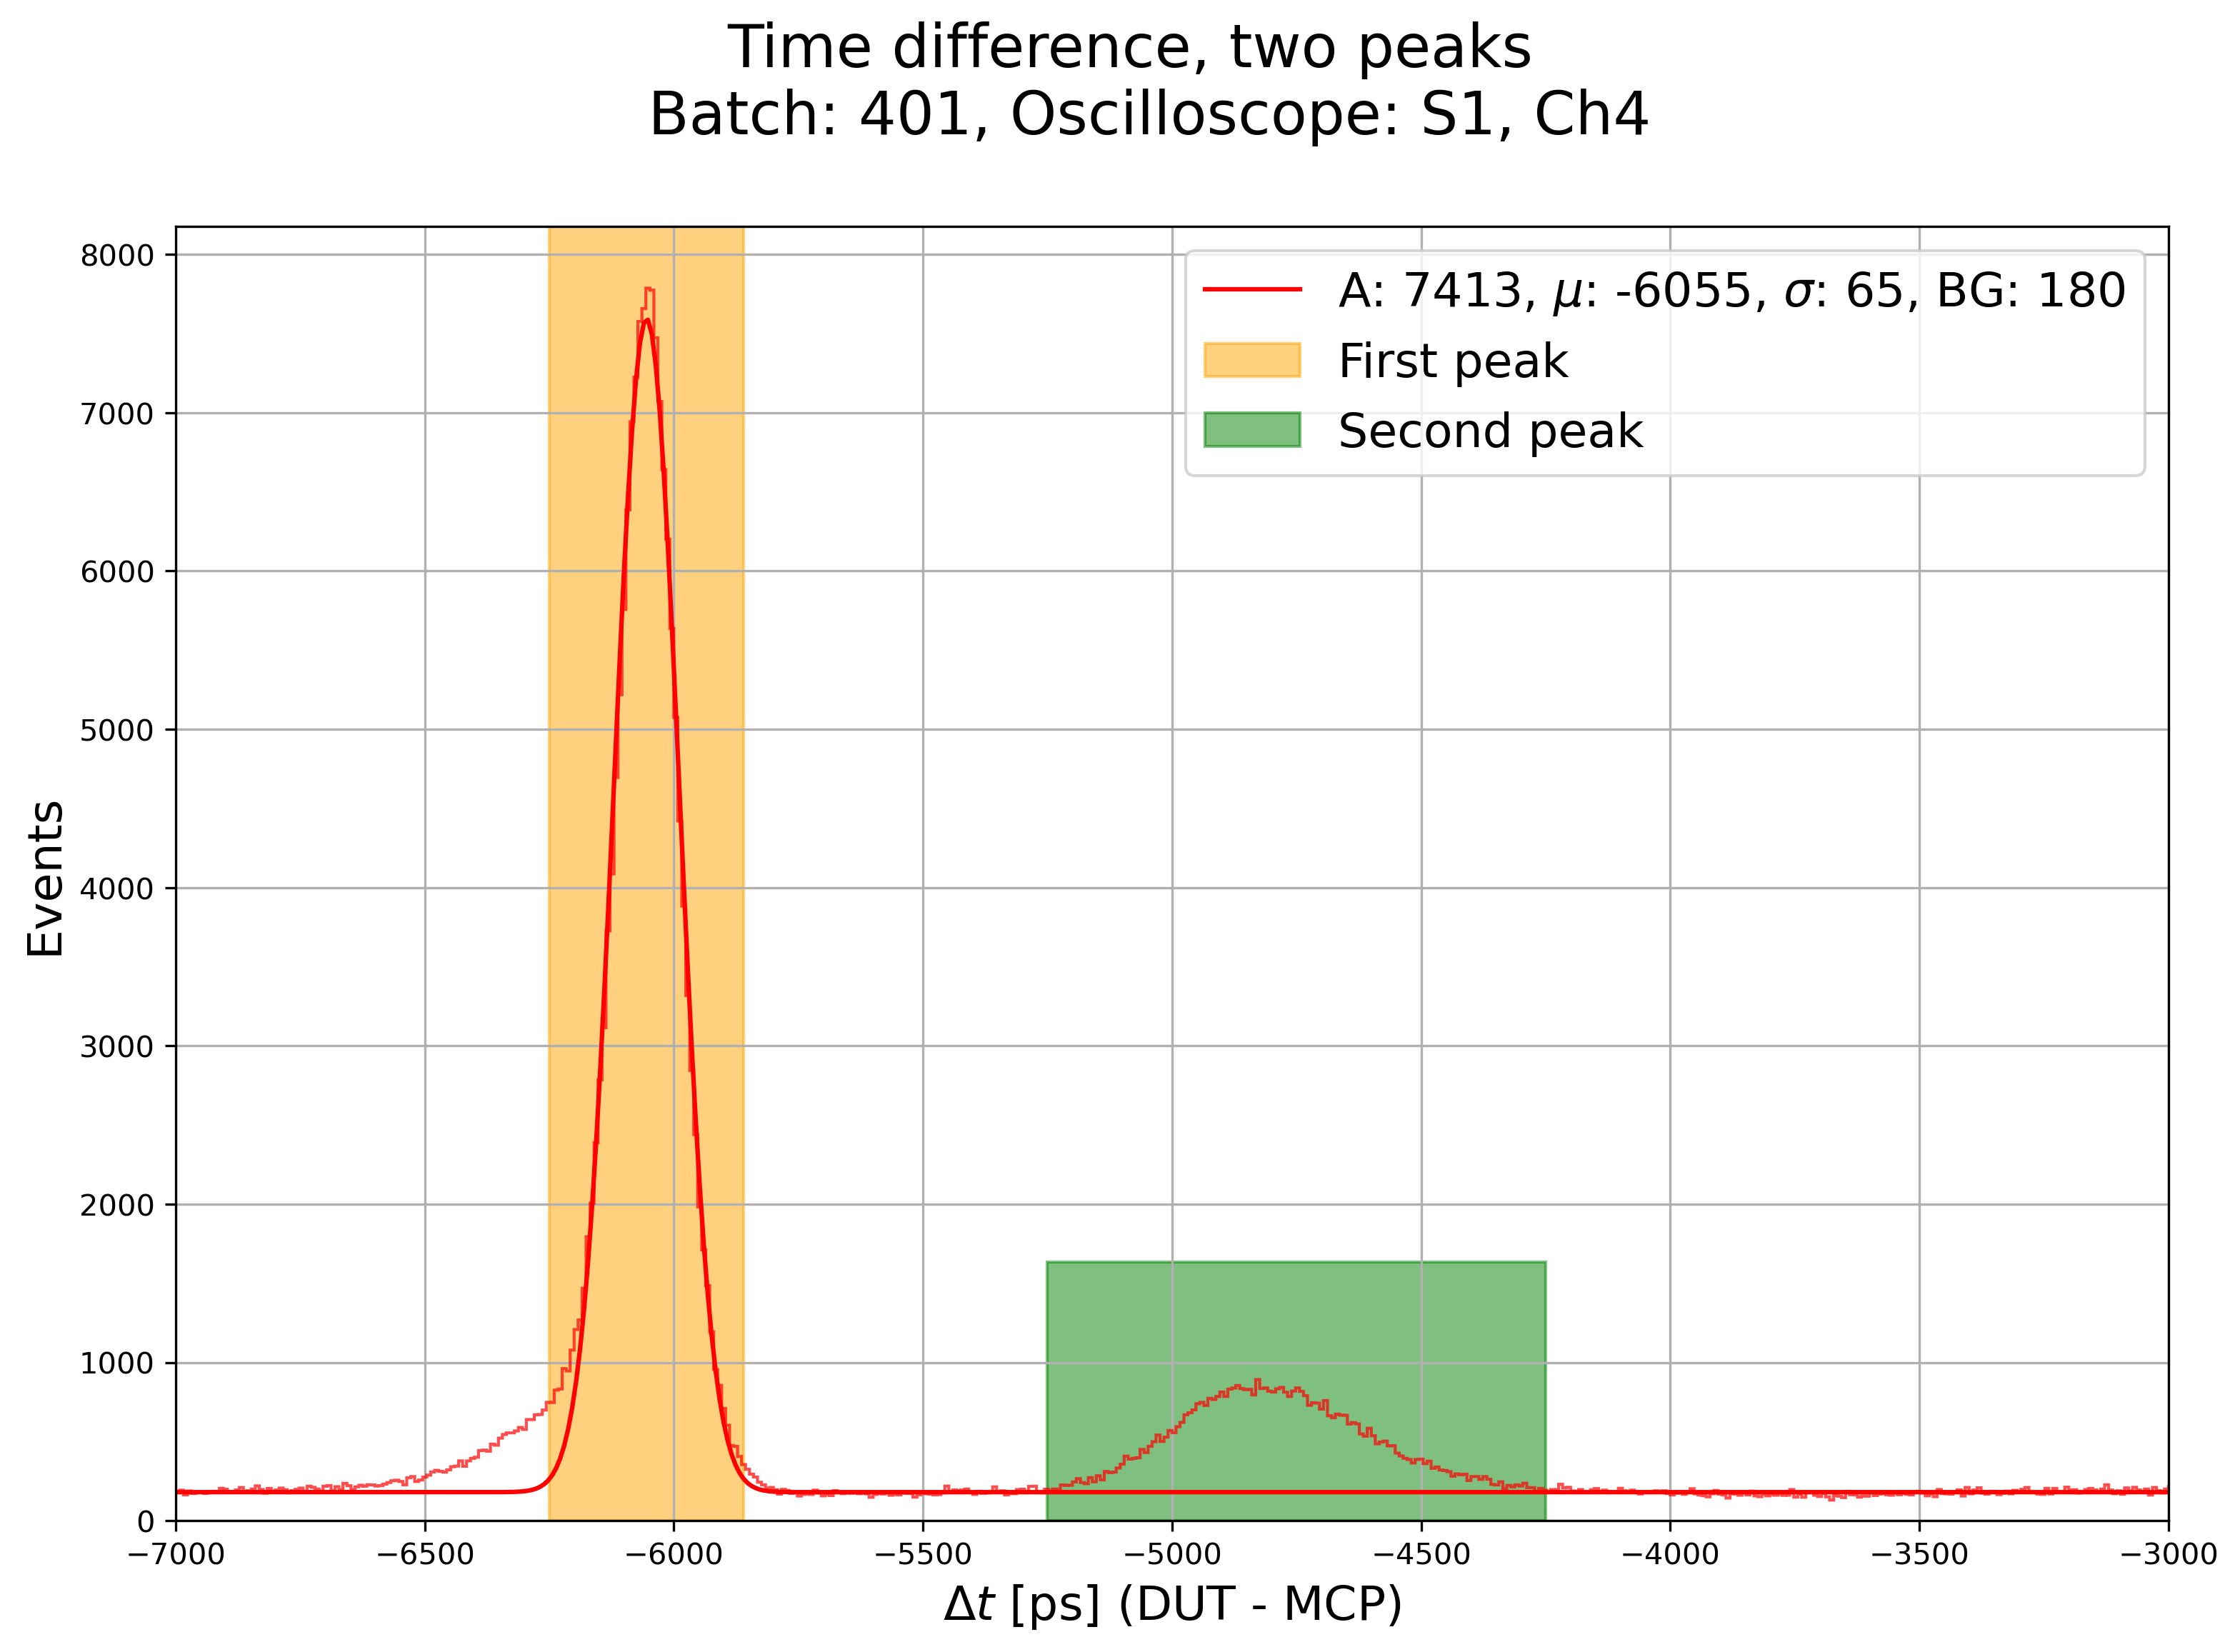
\includegraphics[width=.7\linewidth]{Images/detailed_analysis/time_difference_401_S1_dut_3_with_both_peaks_simple.png}
    \\ [\smallskipamount]
    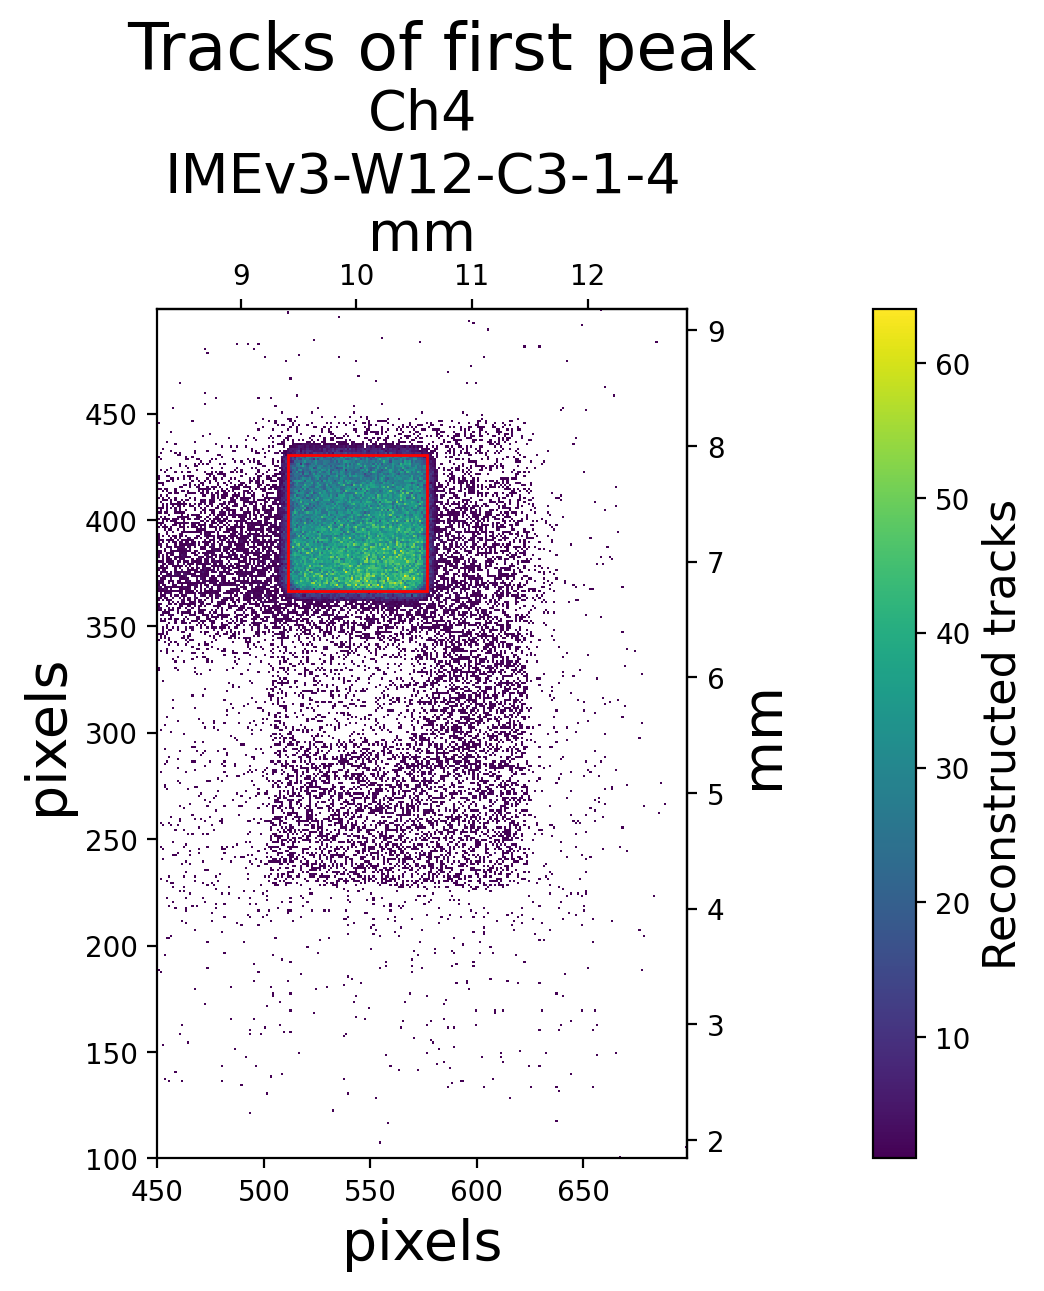
\includegraphics[width=.47\linewidth]{Images/detailed_analysis/2D Tracks 401_S1_dut_3_with_first_peak.png}
    \hfill
    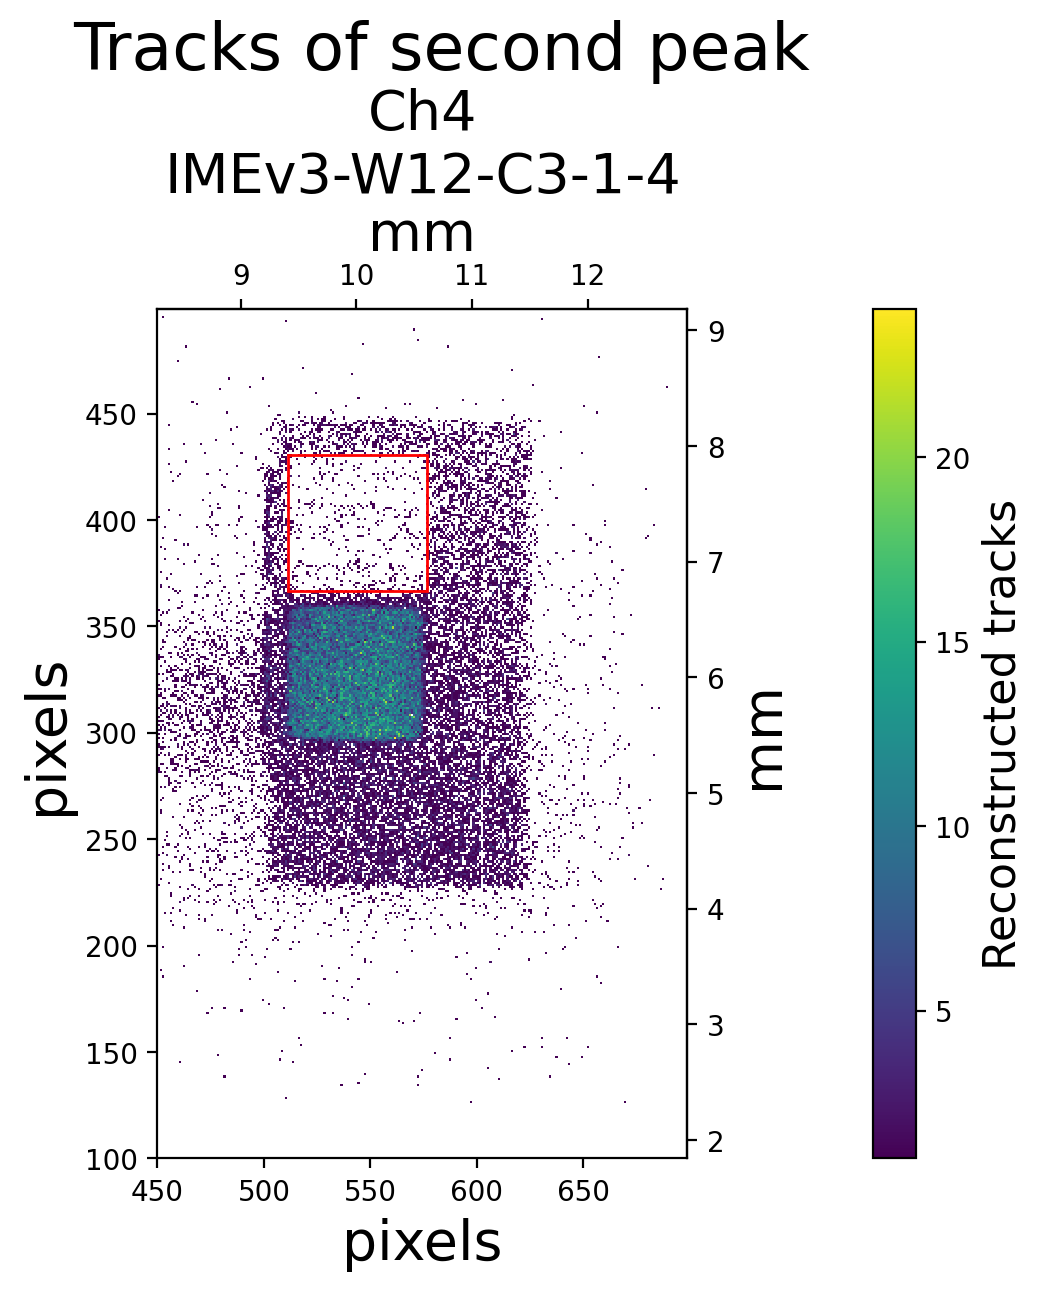
\includegraphics[width=.47\linewidth]{Images/detailed_analysis/2D Tracks 401_S1_dut_3_with_second_peak.png}
    \caption{Top: Time distribution with the first and second peak highlighted in yellow and green, respectively.
    Left: Tracks of events inside yellow interval.
    Right: Tracks of events inside green interval. In red is the outline of the DUT as estimated by the \textit{geometry cut} (\ref{sec:geometry_cut}).}
    \label{fig:time_difference_multiple_peaks_highlight}
\end{figure}
\marginpar{\flushleft Separate the plots so that the text can fit better}


\subsection{Signal from the edges}\label{sec:deviations_from_gaussian}
A secondary effect in the time distribution was the asymmetry between the tails, with the left side notably diverging from a normal distribution. Once again, by singling out only the relevant events, we were able to determine that the ring surrounding the gain layer was responsible for this effect (Figure \ref{fig:time_difference_wide_gaussian}). This further justified our choice of selecting a smaller central area for most of the analysis.

\begin{figure}[!ht]
    \centering
    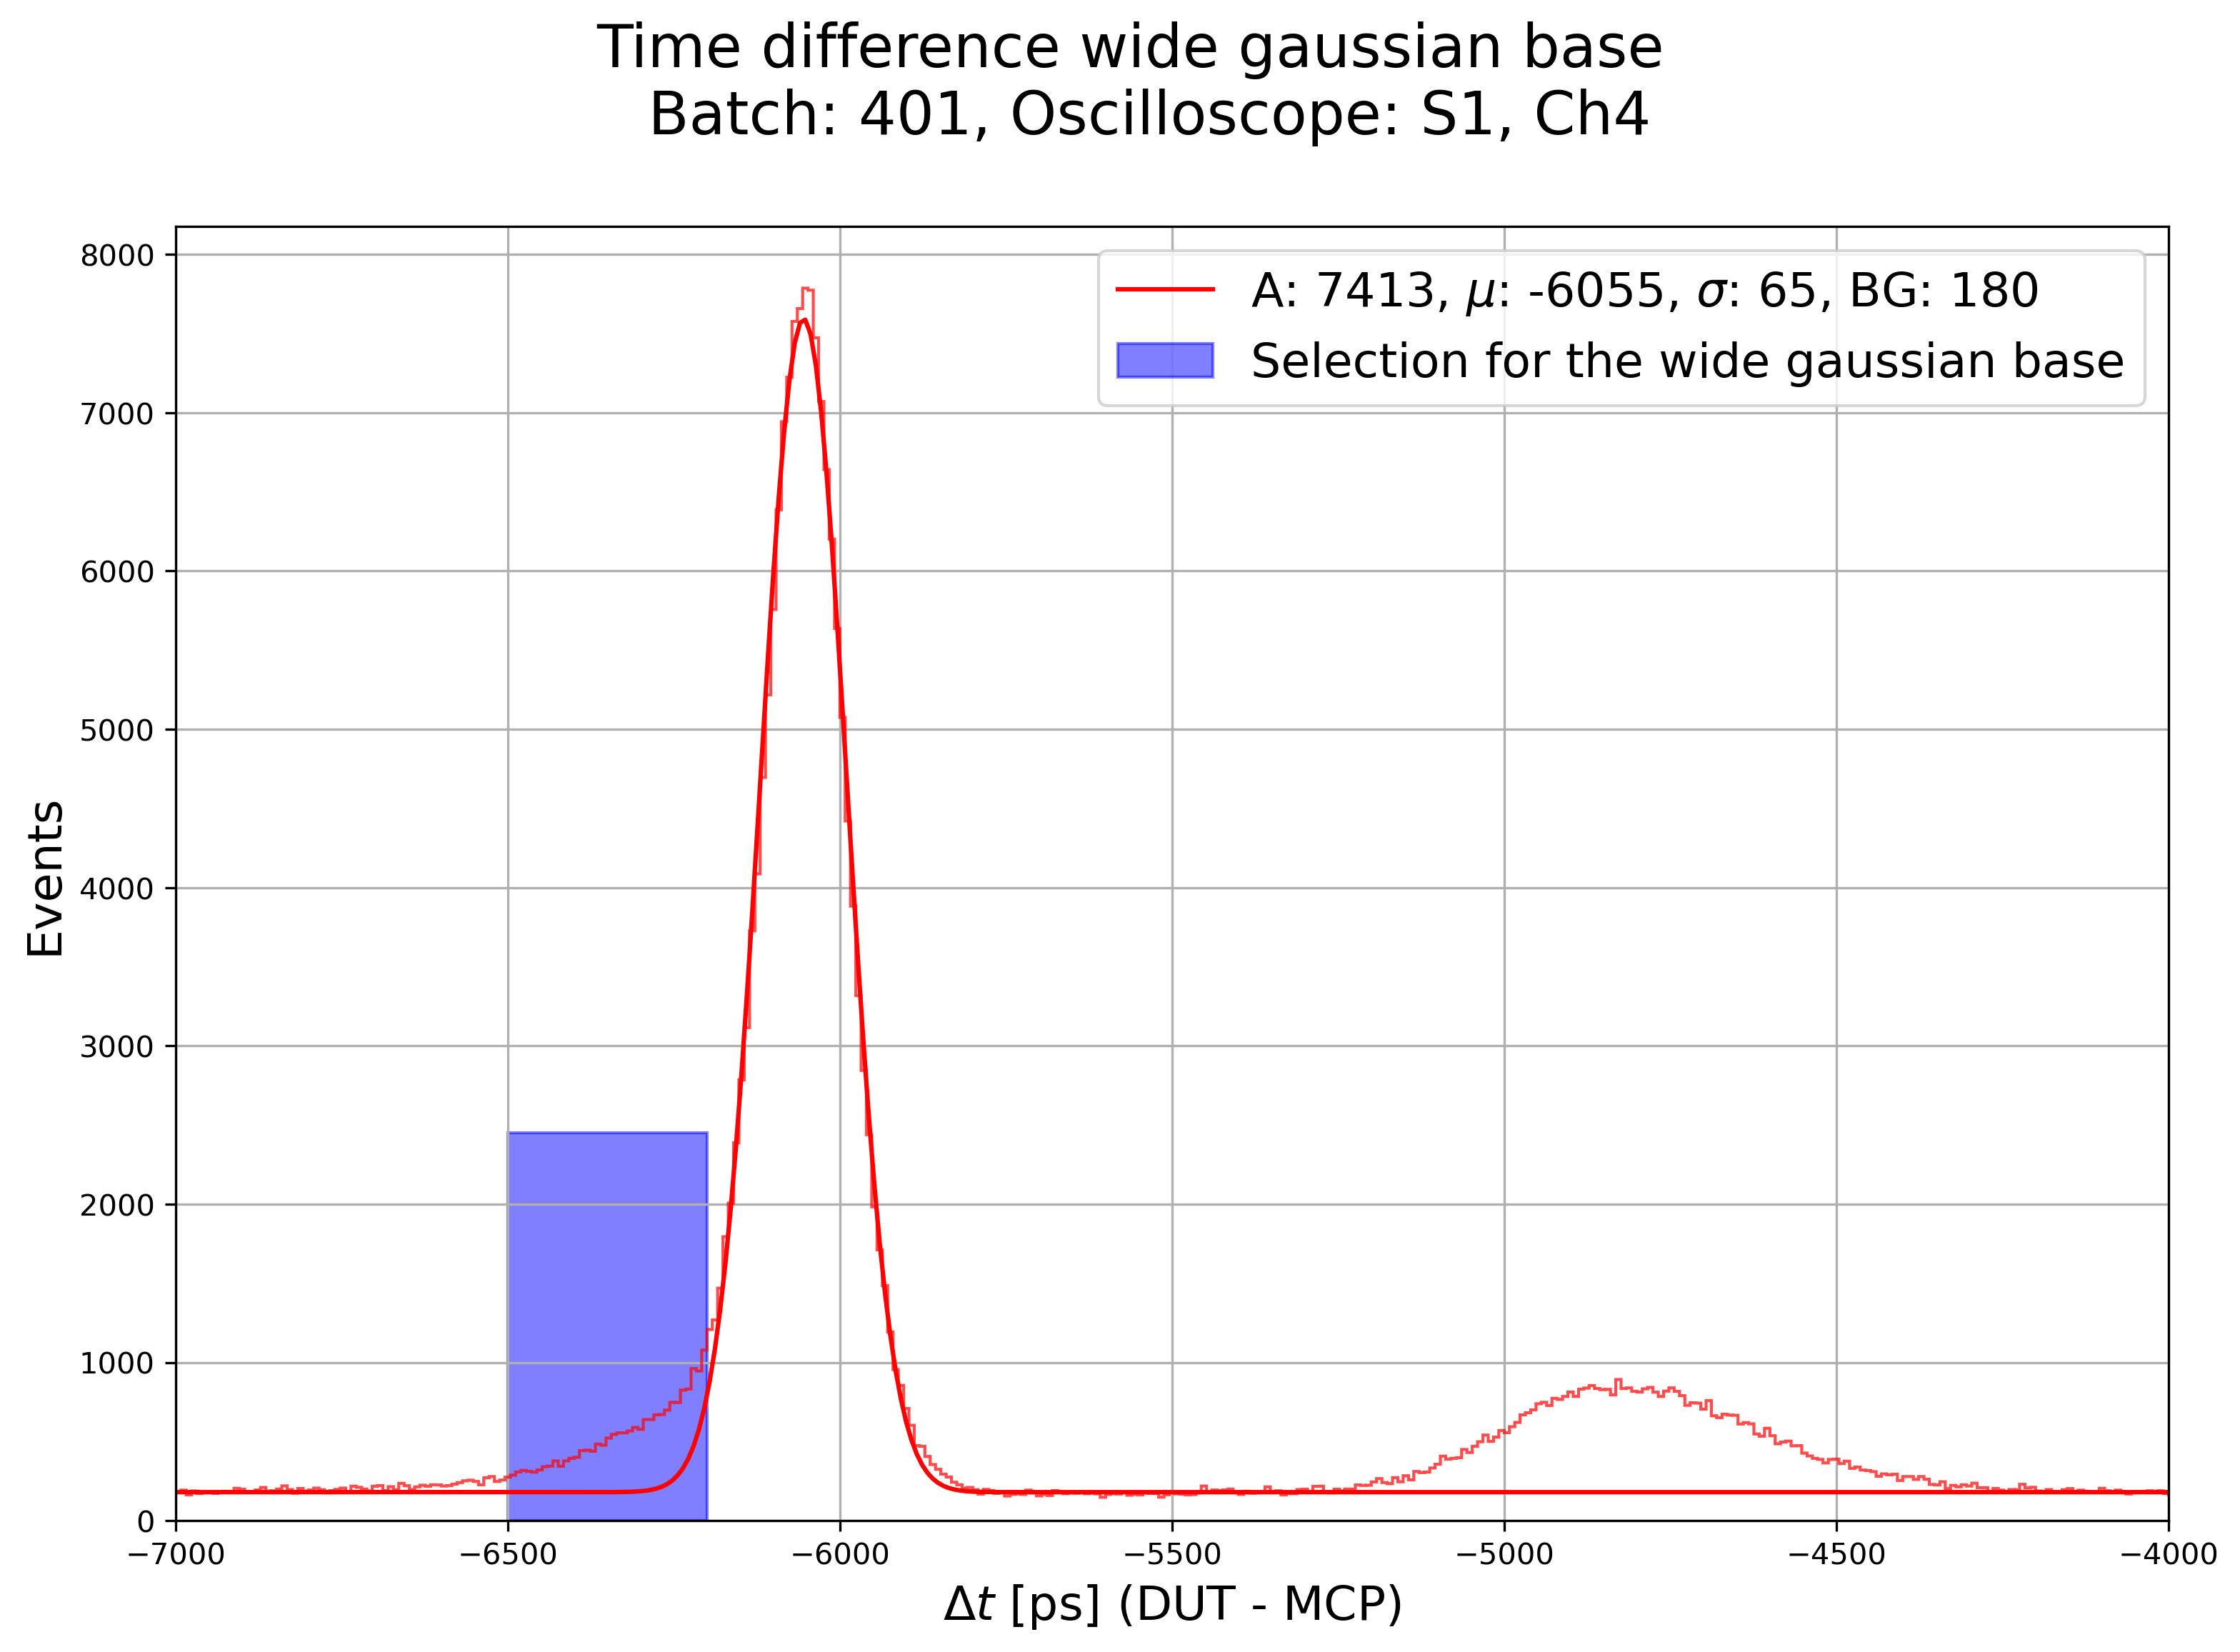
\includegraphics[width=.55\linewidth]{Images/detailed_analysis/time_difference_401_S1_dut_3_with_wide gaussian_left.png}
    \hfill
    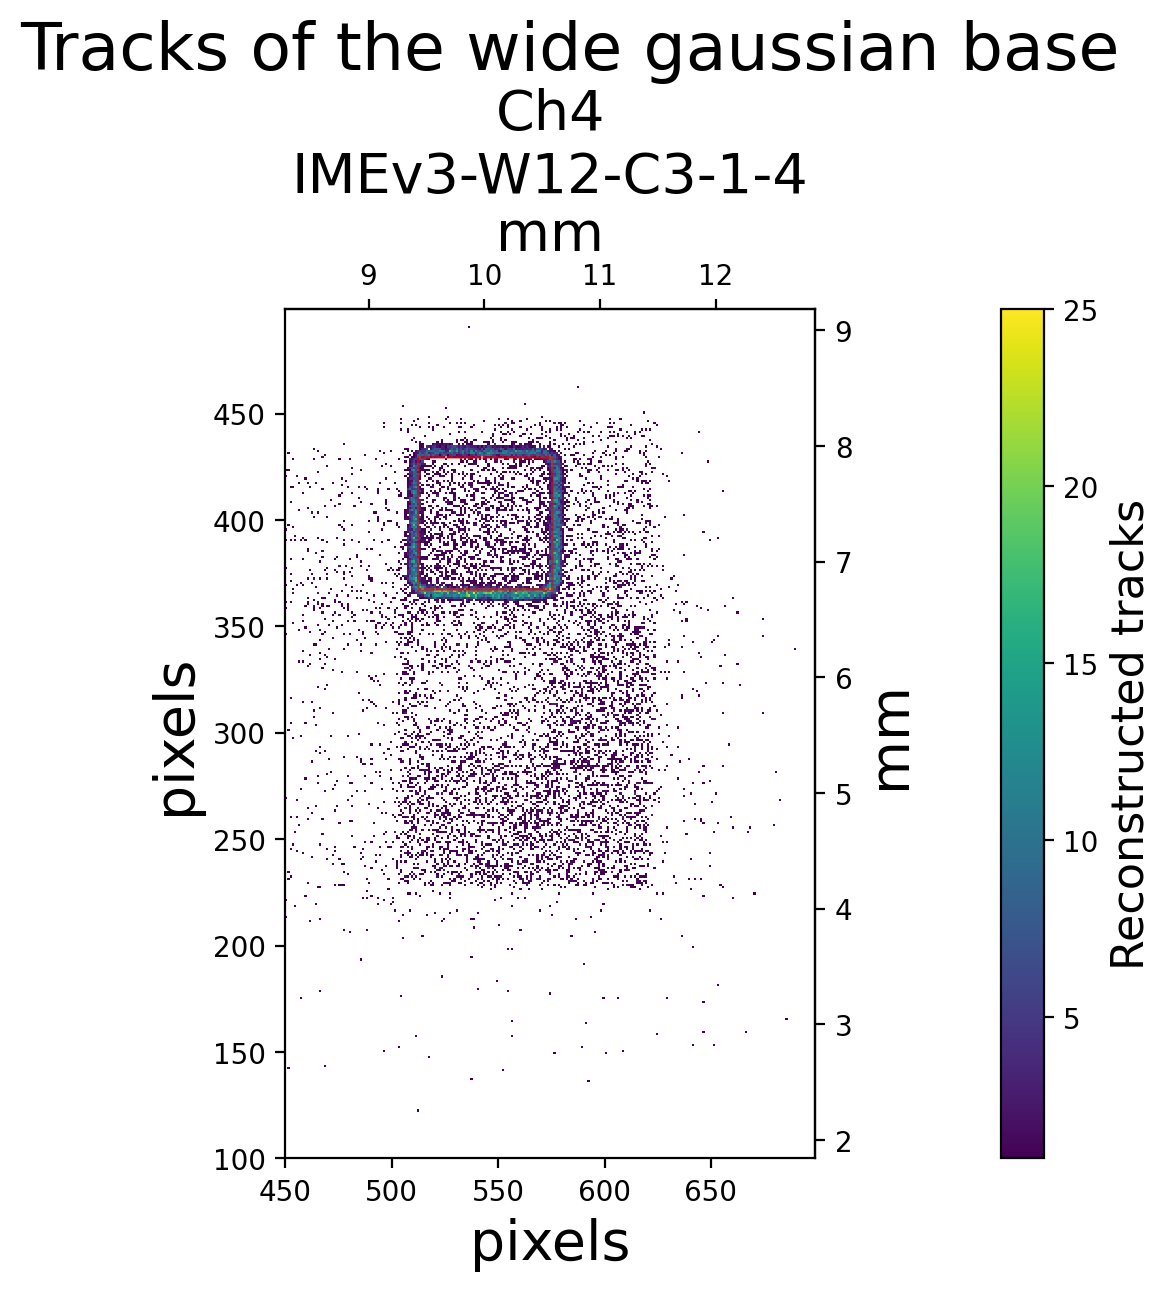
\includegraphics[width=.43\linewidth]{Images/detailed_analysis/2D Tracks 401_S1_dut_3_with_wide_gaussian_base_left.png}
    \caption{Left: selection of the "wide base" of the distribution.
    Right: Tracks of events inside blue interval}
    \label{fig:time_difference_wide_gaussian}
\end{figure}


\subsection{Charge sharing}


\subsection{Pulse clipping}\label{sec:pulse_clipping}

As briefly mentioned before, there was indirect evidence that the pulses recorded by the oscilloscopes had been "cut" at their highest point. To prove this, the waveforms data was investigated, and a sample is shown in Figure \ref{fig:clipped_pulse}. The outcomes were:

\begin{itemize}
    \item Anomaly in the pulseHeight distribution (Figure \ref{fig:pulseHeight_cut})
    \item irregularities in the charge distribution (Figure \ref{fig:charge_vs_pulseHeight_for_clipping})
\end{itemize}
Fortunately, this effect only impacted a small percentage of the data.

\begin{figure}[!ht]
    \centering
    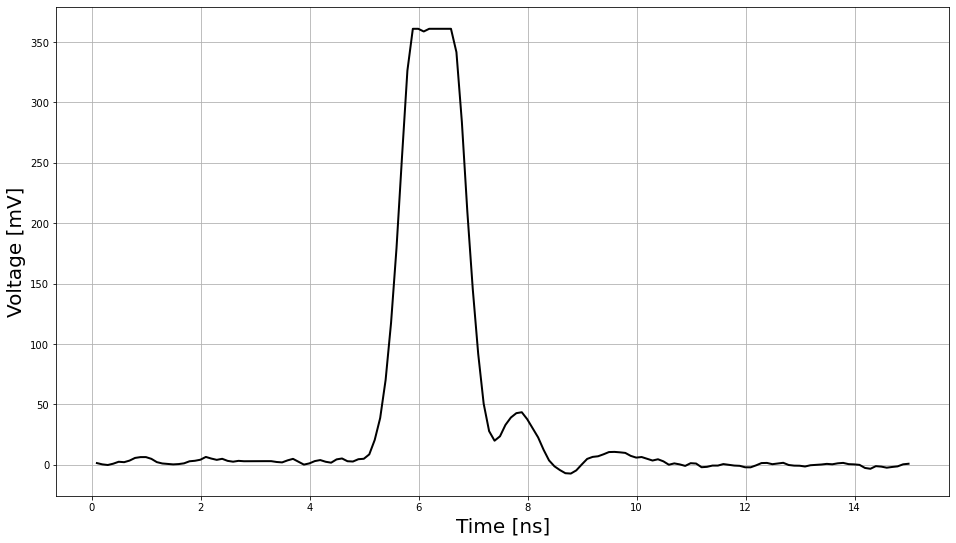
\includegraphics[width=.9\linewidth]{Images/detailed_analysis/Waveform of clipped pulse (ns).png}
    \caption{Example of a single pulse with the highest section cut out}
    \label{fig:clipped_pulse}
\end{figure}
 

\subsubsection{Discrepancies in the tail}\label{subsec:tail_discrepancies}
In a few cases the tail of the distribution deviated considerably from the expected function. We were able to successfully explain this discrepancy with the "clipping" effect in some pulses, due to the limit set to amplitudes registered by the oscilloscopes.
In Section \ref{sec:pulse_clipping} an example of a clipped pulse and its other aftereffects are shown.

In Figure \ref{fig:charge_vs_pulseHeight_for_clipping} (right) the pulseHeight is plotted against the charge and the clipped events appear very clearly at the rightmost part of the plot. This group of events overlapped with the expected charge distribution and could not be removed without modifying it. For this reason, the only solution was to adjust the range of the fit to try to exclude these events.

\begin{figure}
    \centering
    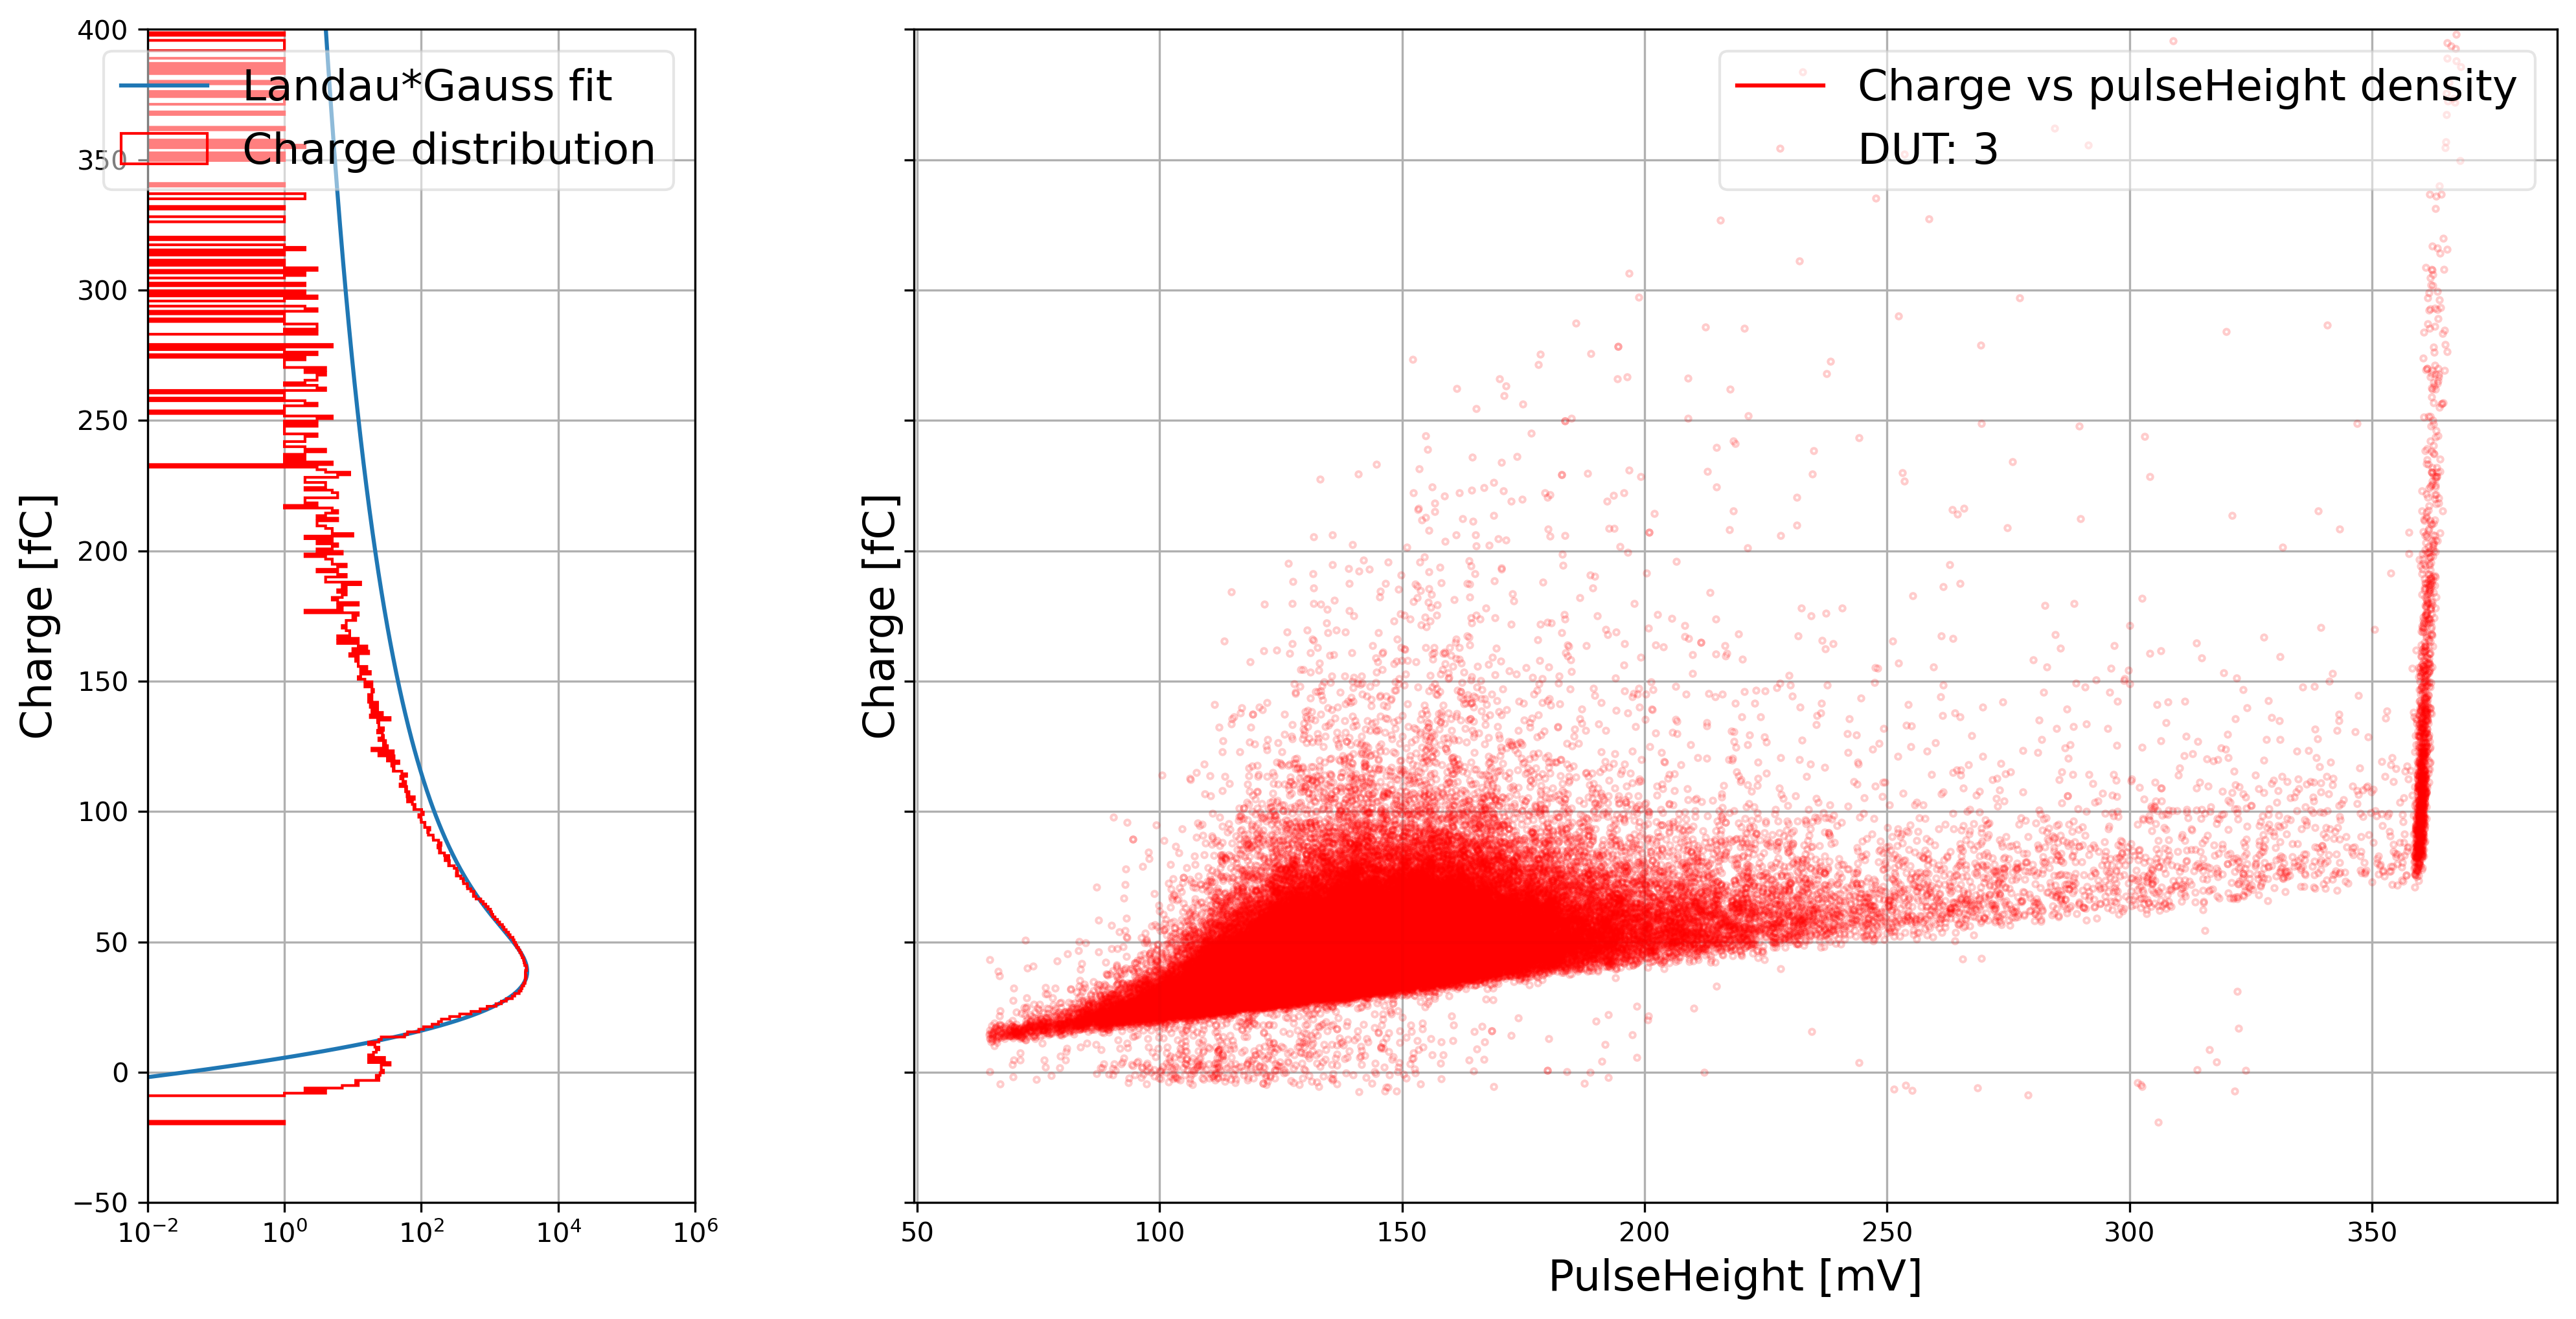
\includegraphics[width=1\linewidth]{Images/charge_plots/Charge_vs_pulseHeight_density_413_S2_dut3.png}
    \caption{Left: distribution of collected charge with Gaussian*Landau fit. Right: scatter plot PulseHeight vs Charge, revealing the cause of the irregular tail}
    \label{fig:charge_vs_pulseHeight_for_clipping}
\end{figure}


\subsection{Temperature fluctuations}\label{sec:temperature_fluctuations}


% \subsection{Charge sharing}\label{sec:charge_sharing}


\subsection{Interpad study}\label{sec:neighbouring_pads}
\begin{figure}
    \centering
    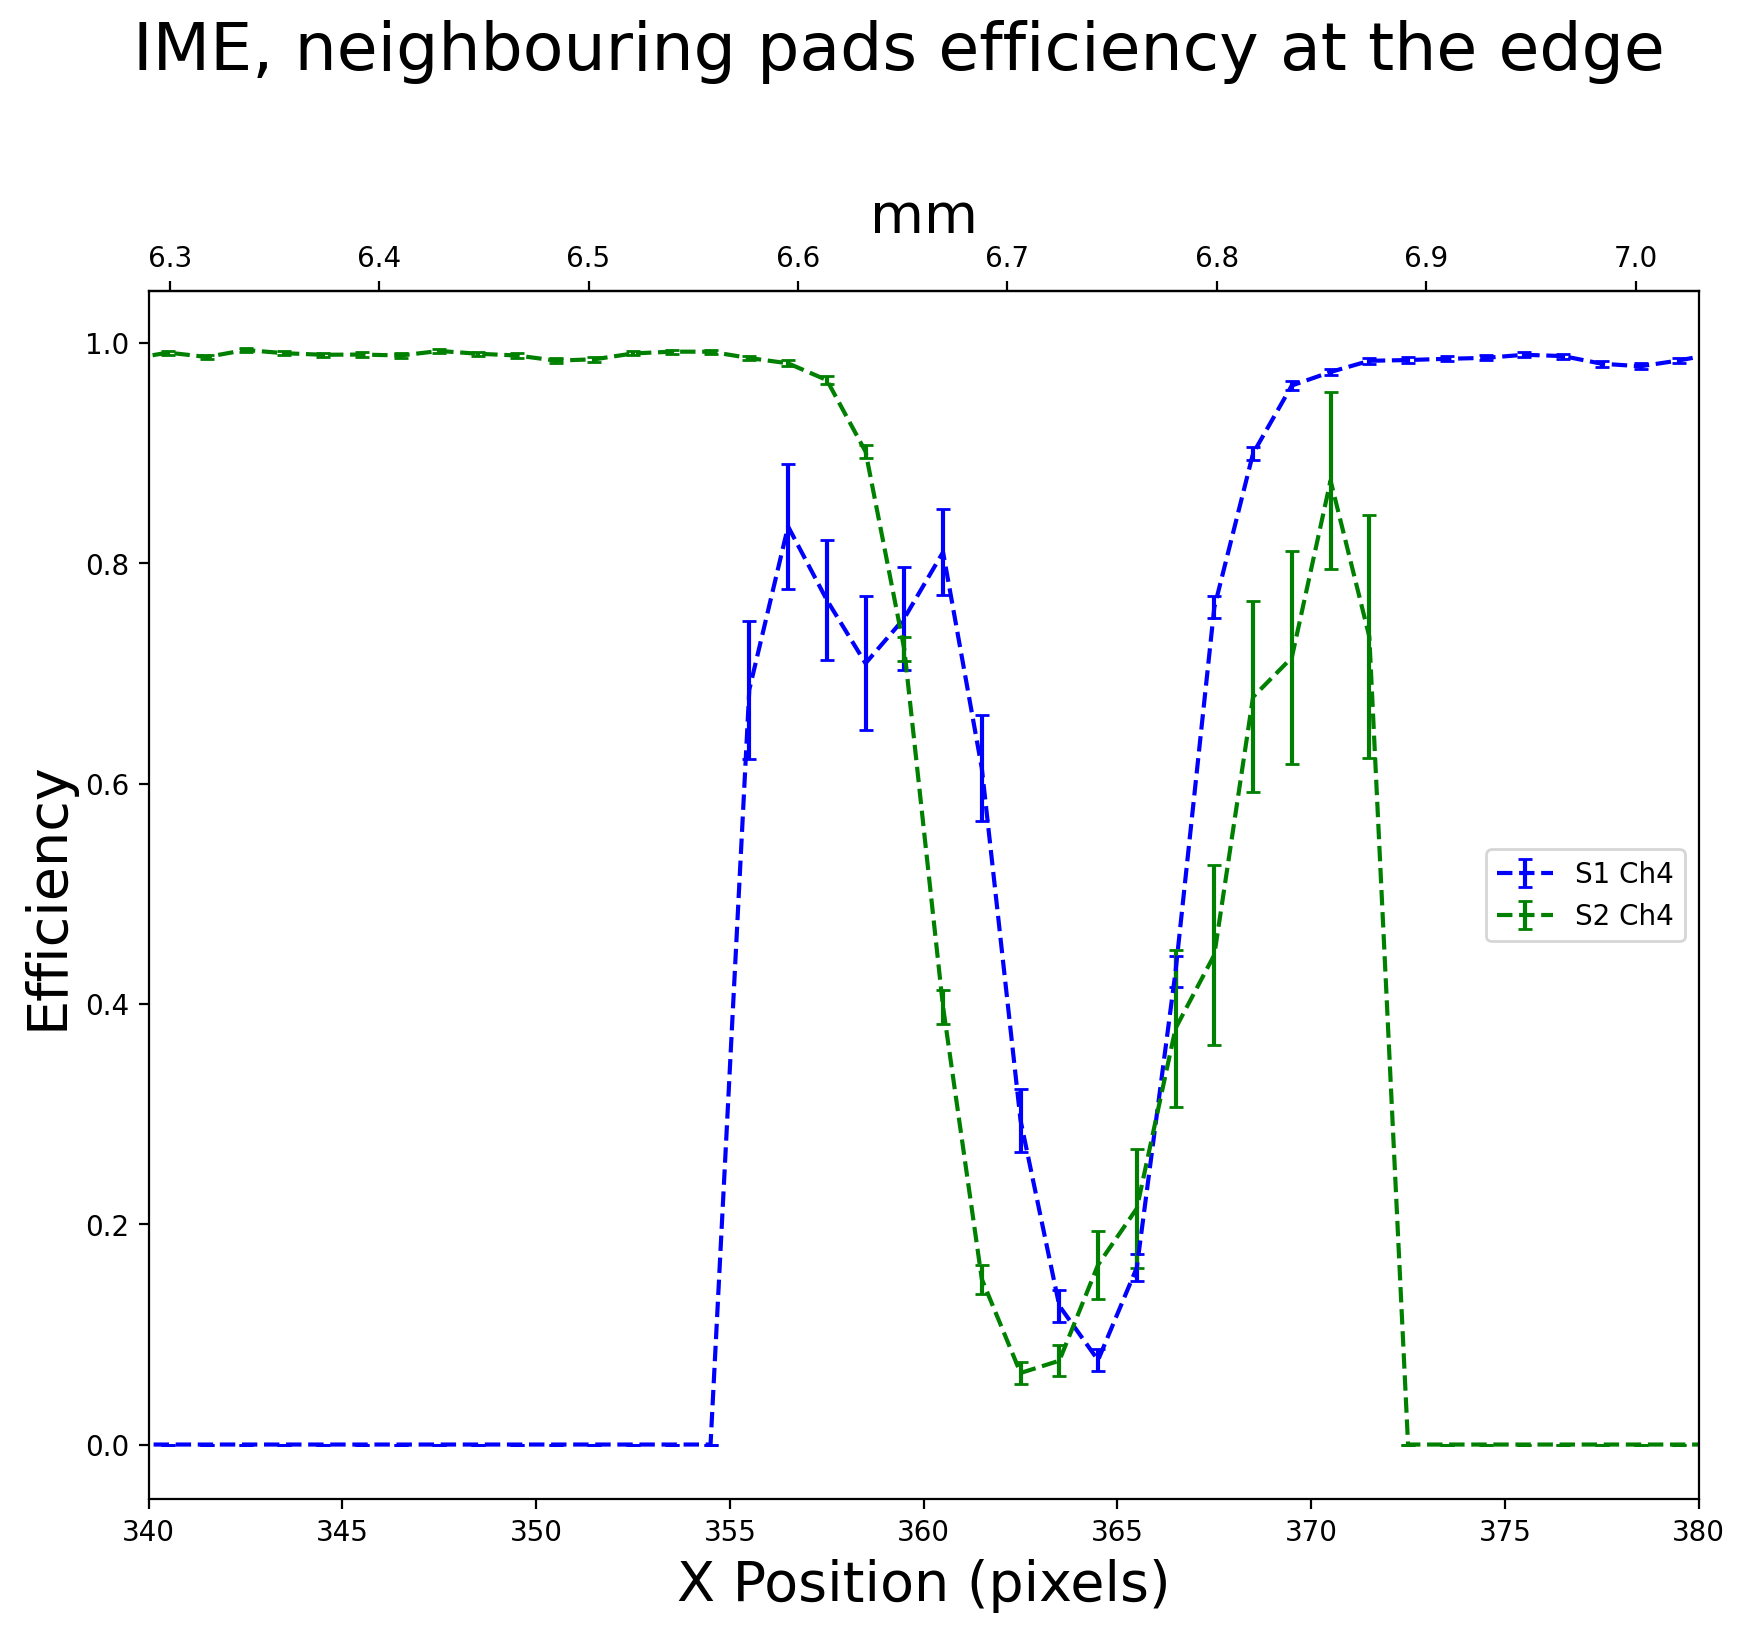
\includegraphics[width=0.5\linewidth]{Images/detailed_analysis/batch 401 duts:3 and 3, edge efficiency studies.png}
    \caption{Caption}
    \label{fig:neighbouring_pads}
\end{figure}
